% ============================================================
% Labor Markets in Chile — BUK Platform Data
% Beamer presentation (work in progress)
% ============================================================
\documentclass[aspectratio=169, 11pt]{beamer}

% ---------- theme & colors ----------
\usetheme{default}
\usecolortheme{default}
\setbeamertemplate{navigation symbols}{}
\setbeamertemplate{footline}[frame number]

% Colors matching academic-pptx palette
\definecolor{navy}{HTML}{1F4E79}
\definecolor{accentblue}{HTML}{2E75B6}
\definecolor{bodytext}{HTML}{2D2D2D}
\definecolor{muted}{HTML}{777777}
\definecolor{lightbg}{HTML}{EBF3FA}
\definecolor{rulecolor}{HTML}{CCCCCC}
\definecolor{faded}{HTML}{BBBBBB}
\definecolor{midblue}{RGB}{46, 117, 182}


\setbeamercolor{frametitle}{fg=navy}
\setbeamercolor{title}{fg=navy}
\setbeamercolor{normal text}{fg=bodytext}
\setbeamercolor{structure}{fg=accentblue}
\setbeamercolor{itemize item}{fg=accentblue}
\setbeamercolor{itemize subitem}{fg=muted}

\setbeamerfont{frametitle}{series=\bfseries, size=\large}
\newcommand{\bmark}[1]{\textcolor{midblue}{\textbf{#1}}}

% ---------- frametitle rule ----------
\setbeamertemplate{frametitle}{%
  \vspace{0.3cm}%
  {\usebeamerfont{frametitle}\usebeamercolor[fg]{frametitle}\insertframetitle}\\[-4pt]%
  {\color{rulecolor}\rule{\textwidth}{0.4pt}}%
  \vspace{0.05cm}%
}

% ---------- packages ----------
\usepackage{booktabs}
\usepackage{graphicx}
\usepackage{hyperref}
\usepackage{amsmath,amssymb}
\usepackage{tikz}
\usetikzlibrary{positioning, arrows.meta, decorations.pathreplacing}
\usepackage[T1]{fontenc}
\usepackage{lmodern}
\usepackage{bbm}
\usepackage{comment}


% ============================================================
\title{Labor Markets in Chile:\\Evidence from Administrative HR Platform Data}
\author{Sofia Valdivia}
\institute{Duke University}
\date{\today}

\begin{document}

% ============================================================
% SLIDE 1: Title
% ============================================================
{
\setbeamercolor{background canvas}{bg=white}
\begin{frame}[plain]
\vfill
\begin{center}
{\Large\bfseries\textcolor{navy}{Market Power and the Gender Career Gap}}\\[6pt]
{\large\textcolor{navy}{Evidence from Matched HR Records in Chile}}\\[20pt]
{\normalsize\textcolor{navy}{Sofia Valdivia}}\\[4pt]
{\small\textcolor{navy}{Duke University}}\\[16pt]
{\small\textcolor{navy}{\today}}
\end{center}
\vfill
\end{frame}
}

% ============================================================
% SLIDE 2: Motivation — Firm-side dynamics (original)
% ============================================================

\begin{frame}
\frametitle{Firms shape careers through hiring and promotion}

\begin{itemize}
    \item \textbf{The gap:} Gender gap research focuses on wages, but firms also decide who to hire and promote. How does labor market power distort these decisions by gender?

    \medskip
    \item \textbf{At hiring:} Audit studies document callback gaps (Bertrand \& Mullainathan, 2004), but cannot observe the full pipeline or link screening to firm characteristics. \bmark{Do firms with more market power screen more aggressively against women?}

    \medskip
    \item \textbf{At promotion:} The first promotion is where the pipeline narrows most (Benson et al., 2026), but evidence is single-firm. \bmark{If women have fewer outside options, firms can extract rents through slower career progression.}

    \medskip
    \item \textbf{This paper:} tests whether firms with greater labor market power distort career dynamics for women at \emph{both} margins.
\end{itemize}

%\vfill
%{\scriptsize\textcolor{muted}{Webber (2016, \textit{JOLE}); Sharma (2023, \textit{JPE}); Benson et al.\ (2024, \textit{QJE}); Cassidy et al.\ (2016, \textit{ILRR}); Bertrand \& Mullainathan (2004, \textit{AER}).}}

\end{frame}

% ============================================================
% SLIDE 4: Chile context
% ============================================================

\begin{frame}
\frametitle{The puzzle of Chile: low participation, persistent wage gaps}

\begin{itemize}
    \item Women surpassed men in education, TFR fell to 1.2, yet the wage gap persists (15--20\%) and female labor force participation remains low (53\% vs.\ OECD 65\%)

    \medskip
    \item If human capital and fertility can't explain the gap, what can? $\Rightarrow$ \textbf{Firm-side frictions:} how firms hire, promote, and retain workers

    \medskip
    \item Chile is also a \textbf{natural laboratory} --- overlapping reforms create variation:
    \begin{itemize}
        \item 40-hour workweek (Ley 21.561) --- changes the cost of ``greedy jobs''
        \item Flexible work for caregivers (Ley 21.645) --- shifts women's outside options
        \item Childcare mandate at 20 female workers (Art.\ 203) --- RD at a firm-size threshold
    \end{itemize}

    \medskip
    \item Each reform (ideally) shifts a \textbf{parameter of the model}: $\lambda_F$ (outside options), hours norms, or the cost of female labor 
\end{itemize}

\end{frame}

% ============================================================
% SLIDE 4: BUK platform data
% ============================================================
\begin{frame}[label=bukslide]
\frametitle{BUK records the full HR pipeline }

\textbf{BUK} is an HR platform used by 19,000+ Chilean firms (4.7M workers, 2022--2026). It records each stage of the employment relationship:

\vspace{0.3cm}
\begin{center}
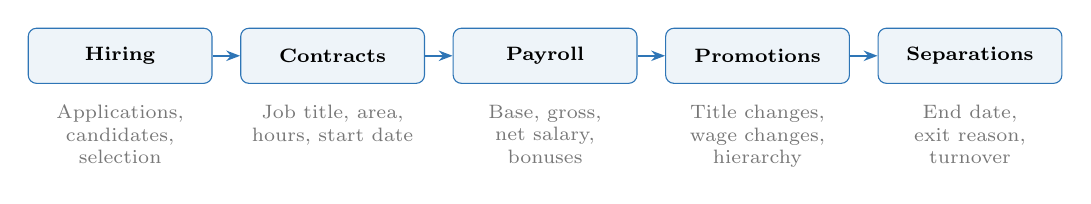
\begin{tikzpicture}[node distance=0.15cm and 0.35cm,
  box/.style={draw=accentblue, rounded corners=3pt, fill=accentblue!8,
              text width=2.1cm, align=center, minimum height=0.7cm, font=\scriptsize\bfseries},
  sub/.style={text width=2.1cm, align=center, font=\scriptsize\color{muted}},
  arr/.style={-{Stealth[length=5pt]}, thick, accentblue}]
  \node[box] (hire) {Hiring};
  \node[box, right=of hire] (contract) {Contracts};
  \node[box, right=of contract] (pay) {Payroll};
  \node[box, right=of pay] (promo) {Promotions};
  \node[box, right=of promo] (exit) {Separations};
  \draw[arr] (hire) -- (contract);
  \draw[arr] (contract) -- (pay);
  \draw[arr] (pay) -- (promo);
  \draw[arr] (promo) -- (exit);
  % sublabels
  \node[sub, below=of hire] {Applications,\\candidates,\\selection};
  \node[sub, below=of contract] {Job title, area,\\hours, start date};
  \node[sub, below=of pay] {Base, gross,\\net salary,\\bonuses};
  \node[sub, below=of promo] {Title changes,\\wage changes,\\hierarchy};
  \node[sub, below=of exit] {End date,\\exit reason,\\turnover};
\end{tikzpicture}
\end{center}

\vspace{0.2cm}
\begin{itemize}
    \item \textbf{Worker--month panel} with firm, occupation, and supervisor identifiers
    \item \textbf{Recruitment:} 186K selection processes, 2.7M applications
    \item \textbf{Complemented by} the Work in Progress survey (perceptions, satisfaction, preferences) \hyperlink{survey}{\beamergotobutton{Survey details}}
\end{itemize}

%\vfill
%{\scriptsize\textcolor{muted}{Data accessed via Delta Sharing. All identifiers anonymized.}}

\end{frame}

% ============================================================
% SLIDE 5: Summary statistics — Firms
% ============================================================
\begin{frame}
\frametitle{Firms: 19,000+ Chilean firms, skewed toward large employers}

\begin{center}
\small
\begin{tabular}{@{}lrr@{}}
\toprule
& \textbf{N firms} & \textbf{\% of workers} \\
\midrule
Large ($>$250 employees) & 5,459 \;\;(28.4\%) & 79.8\% \\
Medium (50--250) & 6,127 \;\;(31.9\%) & 14.5\% \\
Small ($<$50) & 7,612 \;\;(39.6\%) & 5.7\% \\
\midrule
\textbf{Total} & \textbf{19,358} & \textbf{100\%} \\
\bottomrule
\end{tabular}
\end{center}
% check the number of men and women in workers
\vspace{0.3cm}
\begin{itemize}
    \item Panel covers 2022--2026; firm count grows from 6,508 (2022) to 19,104 (2026)
    \item 20 SII economic sectors represented; top 5: retail, professional services, admin services, finance, manufacturing
    \item Linkable to SII tax records for 87\% of firms (sector, sales bracket, equity)
\end{itemize}

%\vfill
%{\scriptsize\textcolor{muted}{Source: BUK platform data. Size classification follows SII brackets.}}

\end{frame}

% ============================================================
% SLIDE 6: Summary statistics — Workers & Jobs
% ============================================================
\begin{frame}
\frametitle{Workers: 4.7M employees with detailed job spells and wage records}

\begin{center}
\small
\begin{tabular}{@{}lr@{}}
\toprule
Unique workers & 4,712,667 \\
Job spells & 8,273,604 \\
Male / Female & 62.8\% / 37.2\% \\
\midrule
\multicolumn{2}{@{}l}{\textit{Job spells per worker}} \\[2pt]
Mean   & 5.86 \\
Median & 3.00 \\
P10    & 1.00 \\
P90    & 14.00 \\
\bottomrule
\end{tabular}
\end{center}

\vspace{0.3cm}
\begin{itemize}
    \item \textbf{Hierarchy:} supervisor link enables org structure and promotion analysis
    \item \textbf{Wages:} base, gross, and net salary; allows fixed vs.\ variable decomposition
    \item \textbf{Job characteristics:} area/occupation, contract type, workday type
    \item \textbf{Separations:} end date for 83.2\% of completed spells; exit reason coverage low
\end{itemize}

%\vfill
%{\scriptsize\textcolor{muted}{Source: BUK platform data, Chile. Coverage rates refer to non-null share in the job table.}}

\end{frame}

% ============================================================
% SLIDE 7: Summary statistics — Recruitment
% ============================================================
\begin{frame}
\frametitle{Recruitment: 186K hiring processes with full application-to-hire pipeline}

\begin{center}
\small
\begin{tabular}{@{}lr@{}}
\toprule
Selection processes & 186,457 \\
Applications & 2,725,982 \\
Unique candidates & 1,146,914 \\
\midrule
Median apps per vacancy & 2 \\
Mean apps per vacancy & 18.7 \\
P90 apps per vacancy & 42 \\
\midrule
Candidate gender: Male / Female & 54.5\% / 44.5\% \\
\bottomrule
\end{tabular}
\end{center}

\vspace{0.3cm}
\begin{itemize}
    \item 68.9\% of processes closed (hired); 48.3\% are replacements, 38.8\% new vacancies
    \item Top referral sources: external portals (40.5\%), company portal (23.7\%), job boards (14.7\%)
    \item Heavy right tail in selectivity --- some vacancies attract 1,000+ applicants 
    % 94 vacancies (0.06%) have more than a thousand, 440 (0.3%) have more than 500. 5912 (4.06%) have more than a 100 apps, 12494 (8.58%) have more than 50 apps
\end{itemize}

%\vfill
%{\scriptsize\textcolor{muted}{Source: BUK platform data, Chile. Candidate gender available for 64.8\% of candidates.}}

\end{frame}



% ============================================================
% SLIDE 9: Research directions
% ============================================================
\begin{frame}
\frametitle{Many possible research questions}

\begin{enumerate}
    \item \textbf{The broken rung at first promotion} 
    \begin{itemize}
        \item Is there a gender gap at the first promotion, and what worker and firm characteristics predict it?
        \item Do firms and workers sort on availability rather than productivity? Do long-hours norms explain who gets promoted?
    \end{itemize}
    \medskip
    \item \textbf{Monopsony power and career dynamics}
    \begin{itemize}
        \item Do firms with greater labor market power offer fewer promotion opportunities to women?
        \item Do firms with greater labor market power screen out women or offer lower entry wages?
    \end{itemize}
    \medskip
    \item \textbf{Firms adjust to mandate cost} 
    \begin{itemize}
        \item How do firms reorganize their workforce in response to mandates? Do they reclassify contract type, substitute towards to male labor, outsource roles?
    \end{itemize}
    \item \textbf{And many more...}
\end{enumerate}

%\vfill
%{\small\textcolor{accentblue}{Next step: narrow to one question and develop identification strategy.}}
%  "Monopsony power and the broken rung." It asks: do firms with greater labor market power have larger gender promotion 
% gaps, particularly at the first rung? Uses application data for monopsony, boss_id for promotions. Connects two major literatures
% that have never intersected. Clear identification (variation in local labor market concentration across occupation x region). High feasibility — doesn't depend on is_parent.
\end{frame}

% ============================================================
% SLIDE 10: Highlight — Monopsony power
% ============================================================
\begin{frame}
\frametitle{Many possible research questions}

\begin{enumerate}
    \item \textcolor{faded}{The broken rung at first promotion}
    \begin{itemize}
        \item \textcolor{faded}{Is there a gender gap at the first promotion, and what worker and firm characteristics predict it?}
        \item \textcolor{faded}{Do firms and workers sort on availability rather than productivity? Do long-hours norms explain who gets promoted?}
    \end{itemize}
    \medskip
    \item \textbf{\textcolor{navy}{Monopsony power and career dynamics}}
    \begin{itemize}
        \item Do firms with greater labor market power offer fewer promotion opportunities to women?
        \item Do firms with greater labor market power screen out women or offer lower entry wages?
    \end{itemize}
    \medskip
    \item \textcolor{faded}{Firms adjust to mandate cost}
    \begin{itemize}
        \item \textcolor{faded}{How do firms reorganize their workforce in response to mandates? Do they reclassify contract type, substitute towards male labor, outsource roles?}
    \end{itemize}
        \item \textcolor{faded}{And many more...}

\end{enumerate}

\end{frame}



% ============================================================
% SLIDE 11 (alt): Literature — streamlined version
% ============================================================
\begin{frame}
\frametitle{Two literatures have developed in parallel --- this paper connects them}

\begin{itemize}
    \item \textbf{Monopsony $\times$ gender:} market power depresses women's wages (Webber, 2016; Sharma, 2023); outside options causally shape within-firm outcomes (Caldwell \& Danieli, 2022) --- \small \bmark{but only studied for \emph{wages}}
    \normalsize
    \medskip
    \item \textbf{Gender $\times$ career dynamics:} promotion gaps persist after controlling for performance (Benson et al., 2026); hiring discrimination documented via audits (Bertrand \& Mullainathan, 2004) --- \small \bmark{but no connection to \emph{market structure}}
    \normalsize
    \medskip
    \item \textbf{The missing intersection:} Whether market power distorts hiring screening or promotion decisions by gender. %The mechanism: if women have fewer outside options ($\lambda_F < \lambda_M$), firms face less competitive pressure to hire fairly or promote --- 
    Are rents extracted through slower career progression.

    \medskip
    \item \textbf{Contribution:} Connect monopsony to career dynamics at both margins, using application-level data to measure market power directly
\end{itemize}

\end{frame}

% ============================================================
% MODEL SLIDES
% ============================================================

% --- SLIDE 12: Model overview ---
\begin{frame}
\frametitle{Model overview: on-the-job search with hiring and promotion decisions}

\textbf{Building on:} Burdett \& Mortensen (1998) wage-posting search model, extended with an internal promotion decision (Gibbons \& Waldman, 1999) and gender-specific outside options (Sharma, 2023).

\begin{center}
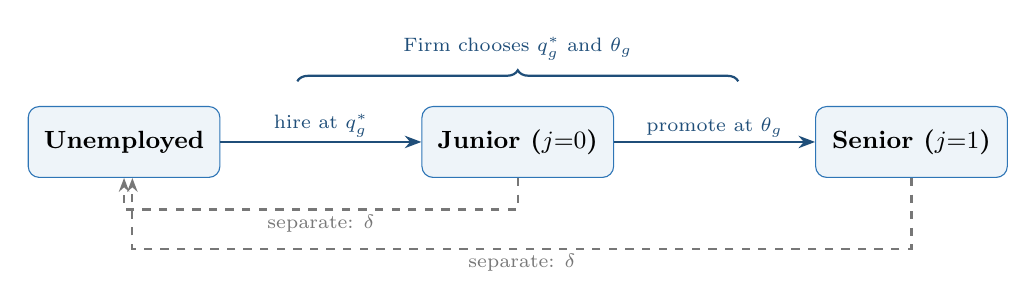
\begin{tikzpicture}[
  state/.style={draw=accentblue, rounded corners=4pt, fill=accentblue!8,
                text width=2.2cm, align=center, minimum height=0.9cm, font=\small\bfseries},
  firm/.style={-{Stealth[length=6pt]}, thick, navy},
  sep/.style={-{Stealth[length=5pt]}, thick, muted, dashed},
  lbl/.style={font=\scriptsize, fill=white, inner sep=1.5pt}]
  % States
  \node[state] (unemp) at (0,0) {Unemployed};
  \node[state] (junior) at (5,0) {Junior ($j{=}0$)};
  \node[state] (senior) at (10,0) {Senior ($j{=}1$)};
  % Forward arrows (firm decisions)
  \draw[firm] (unemp) -- (junior) node[lbl, midway, above] {hire at $q_g^*$};
  \draw[firm] (junior) -- (senior) node[lbl, midway, above] {promote at $\theta_g$};
  % Separation arrows (back to unemployed)
  \draw[sep] (junior.south) -- ++(0,-0.4) -| (unemp.south)
    node[lbl, pos=0.25, below] {separate: $\delta$};
  \draw[sep] (senior.south) -- ++(0,-0.9) -| ([xshift=3pt]unemp.south)
    node[lbl, pos=0.25, below] {separate: $\delta$};
  % Annotations
  %\node[above=0.9cm of junior, font=\scriptsize\color{navy}] {\textbf{Firm chooses}};
  \draw[navy, thick, decorate, decoration={brace, amplitude=4pt, raise=2pt}]
    (2.2,0.7) -- (7.8,0.7) node[midway, above=6pt, font=\scriptsize\color{navy}] {Firm chooses $q_g^*$ and $\theta_g$};
\end{tikzpicture}
\end{center}

\small
\begin{itemize}
    \item Continuous time, two worker types: $g \in \{M, F\}$
    \item Firms heterogeneous in productivity $p \sim F(p)$; two job levels per firm
    \item \textbf{Key parameter:} outside offer arrival rate $\lambda_g$, with $\lambda_F < \lambda_M$
    \item Firms choose \textbf{two instruments}: screening threshold at hiring and promotion threshold
\end{itemize}
% It's NOT about preferring men or limited promotion slots. The model has no fixed number of promotions. Each worker's promotion is an independent cost-benefit decision by the firm. 
\end{frame}


% --- SLIDE 13: Workers' problem ---
\begin{frame}
\frametitle{Workers' problem}

Workers of gender $g$ are either \textbf{unemployed} or \textbf{employed} at level $j \in \{0,1\}$ in a firm of type $p$.

\vspace{0.3cm}
\textbf{Value of unemployment:}
\begin{equation*}
    rU_g = b + \lambda_g^u \int \max\{V_{g0}(w) - U_g,\; 0\} \, dF_g(w)
\end{equation*}

where $b$ is the flow value of unemployment, $\lambda_g^u$ is the offer arrival rate, and $F_g(w)$ is the wage offer distribution.

\vspace{0.3cm}
\textbf{Value of employment at level $j$:}
\begin{align*}
    rV_{gj}(p) = & w_{gj}(p) + \lambda_g \int \max\{V_{g0}(w') - V_{gj}(p),\; 0\} \, dF_g(w') + \delta[U_g - V_{gj}(p)] \\ 
    & + \mathbbm{1}_{j=0} \cdot \mu_g(p)[V_{g1}(p) - V_{g0}(p)] % something that doesnt make sense here is that someone at senior level, if they accpet a job at another firm, will have to start as a junior, would they get paid less?
\end{align*}

\begin{itemize}
    \item $\lambda_g$: on-the-job outside offer arrival rate (\textbf{$\lambda_F < \lambda_M$})
    %\item $\delta$: exogenous separation rate
    \item $\mu_g(p)$: promotion rate at firm $p$ for gender $g$ (determined by firm's choice)
    %\item Workers accept any outside offer that improves lifetime value
\end{itemize}

\end{frame}

% --- SLIDE 14: Firm's problem — setup ---
\begin{frame}
\frametitle{Firm's problem: two instruments}

A firm with productivity $p$ employs workers at two levels. Output of gender-$g$ worker at level $j$:
\begin{equation*}
    y_{j}(p) = p \cdot a_j \qquad \text{with } a_1 > a_0 % senior workers produce more
    % VERY important, I'm not saying there's a prductivity gender differnece, it all comes from firm's side
\end{equation*}

The firm chooses \textbf{four objects} for each gender $g$:

\vspace{0.3cm}
\textbf{Decision 1: Hiring} \textcolor{faded}{(Shi, 2002)}
\begin{itemize}
    \item Entry wage $w_{g0}$ and screening threshold $q_g^*$
    \item Applicants draw quality signal $q \sim H(q)$; hired if $q \geq q_g^*$
    \item Trade-off: higher $q_g^*$ $\to$ better workers, fewer hires
\end{itemize}

\vspace{0.3cm}
\textbf{Decision 2: Promotion} \textcolor{faded}{(Gibbons \& Waldman, 1999)}
\begin{itemize}
    \item Promotion threshold $\theta_g$ and senior wage $w_{g1}$
    \item Each period, junior worker draws performance signal $s \sim G(s)$; promoted if $s \geq \theta_g$
    \item Trade-off: lower $\theta_g$ $\to$ more promotions (higher output), but higher wage bill
    \item \textbf{Retention motive:} promoting prevents separation to outside offers
\end{itemize}

\end{frame}

% --- SLIDE 15: Firm's problem — optimization ---
\begin{frame}
\frametitle{Firm's problem: steady-state profit maximization}

The firm chooses $(w_{g0}, w_{g1}, q_g^*, \theta_g)$ to maximize steady-state profits:

\begin{equation*}
    \pi_g(p) = \sum_{j \in \{0,1\}} \bigl[y_{j}(p) - w_{gj}\bigr] \cdot n_{gj}(p)
\end{equation*}

where the steady-state workforce $n_{gj}(p)$ depends on three flows:

\vspace{0.2cm}
\begin{enumerate}
    \item \textbf{Inflow} (hiring): $h_g(p) = \lambda_g^u \cdot u_g \cdot [1 - H(q_g^*)] \cdot \mathbbm{1}\{V_{g0}(p) \geq U_g\}$
    \medskip
    \item \textbf{Internal flow} (promotion): $\mu_g(p) = 1 - G(\theta_g)$
    \medskip
    \item \textbf{Outflow} (separation): $s_g(p) = \delta + \lambda_g \cdot [1 - F_g(V_{gj}(p))]$
\end{enumerate}

\vspace{0.3cm}
In steady state, the mass at each level satisfies:
\begin{align*}
    \dot{n}_{g0} &= h_g(p) - [\mu_g(p) + s_g(p)] \cdot n_{g0} = 0 \\
    \dot{n}_{g1} &= \mu_g(p) \cdot n_{g0} - s_g(p) \cdot n_{g1} = 0
\end{align*}

\end{frame}

\begin{comment}
% --- SLIDE 16: The retention mechanism ---
\begin{frame}
\frametitle{The retention mechanism: why monopsony distorts promotions}

\textbf{First-order condition for the promotion threshold $\theta_g$:}

\begin{equation*}
    \underbrace{(y_{1} - w_{g1}) - (y_{0} - w_{g0})}_{\text{Marginal profit from promoting}} = \underbrace{\frac{\partial s_g / \partial \theta_g}{\phi(\theta_g)} \cdot n_{g0} \cdot (y_{0} - w_{g0})}_{\text{Retention value of NOT promoting}}
\end{equation*}

\begin{itemize}
    \item \textbf{LHS:} gain from moving worker to the senior level (higher output net of higher wage)
    \medskip
    \item \textbf{RHS:} delaying promotion is costly only if the worker might \emph{leave} --- this depends on $\lambda_g$
    \medskip
    \item When $\lambda_F < \lambda_M$: $\dfrac{\partial s_F}{\partial \theta_F} < \dfrac{\partial s_M}{\partial \theta_M}$

    \vspace{0.2cm}
    $\Rightarrow$ The retention cost of delaying promotion is \textbf{lower for women}

    $\Rightarrow$ Firms optimally set $\theta_F^* > \theta_M^*$ (higher bar for women)
    \medskip
    \item Monopsony power $\Rightarrow$ under-promote women because women are less likely to leave
\end{itemize}

\end{frame}
\end{comment}
% --- SLIDE 16-ALT-A: Retention mechanism — intuitive version ---
\begin{frame}[label=retentionslide]
\frametitle{The retention trade-off: why monopsony distorts promotions}

The firm's promotion decision balances \textbf{two forces}:

\vspace{0.1cm}
\begin{enumerate}
    \item \textbf{Direct profit effect:} promoting changes per-worker surplus

    Output rises ($a_1 > a_0$), but so does the wage ($w_{g1} > w_{g0}$). %The output gain $p(a_1 - a_0)$ is gender-neutral, but the surplus change $\pi_1 - \pi_0$ depends on gender-specific wages.
    \bigskip
    \item \textbf{Retention effect:} promoting makes the worker less likely to leave. Promotion $\to$ $V_{1g} > V_{0g}$ $\to$ fewer outside offers are attractive $\to$ lower separation. %This benefit depends on $\lambda_g$:
\end{enumerate}

\vspace{0.1cm}
\begin{columns}[T]
    \begin{column}{0.45\textwidth}
        \textbf{Men} (high $\lambda_M$):
        \begin{itemize}
            \item ``If I don't promote him, he'll leave''
            \item Retention urgency is \textbf{high}
            \item[$\Rightarrow$] Promote to retain
        \end{itemize}
    \end{column}
    \begin{column}{0.45\textwidth}
        \textbf{Women} (low $\lambda_F$):
        \begin{itemize}
            \item ``Even without promotion, she won't leave''
            \item Retention urgency is \textbf{low}
            \item[$\Rightarrow$] Delay is low-cost
        \end{itemize}
    \end{column}
\end{columns}

\vspace{0.3cm}
$\Rightarrow$ $\theta_F^* > \theta_M^*$: higher bar for women, not from productivity differences, but because firms face \textbf{less competitive pressure} to promote them.
\hfill\hyperlink{foc-formal}{\beamergotobutton{Formal FOC}}

\end{frame}

% --- SLIDE 17: The hiring screening mechanism ---
\begin{frame}
\frametitle{The hiring mechanism: why monopsony distorts screening}

When $\lambda_F < \lambda_M$, two \textbf{opposing forces} shape the firm's screening threshold $q_g^*$:

\vspace{0.3cm}
\begin{enumerate}
    \item \textbf{``Longer tenure'' force} $\to$ screen women \emph{less}

    Women stay longer at the firm $\to$ each hire generates surplus over more periods $\to$ the expected value of a marginal hire is higher $\to$ firm should lower the bar to hire more women

    \bigskip
    \item \textbf{``Less competition'' force} $\to$ screen women \emph{more}

    Women have fewer outside options $\to$ they apply even when the bar is high $\to$ firm can raise $q_F^*$ without losing its applicant pool $\to$ ``cherry-pick''
\end{enumerate}

\vspace{0.3cm}
\textbf{The sign of $q_F^* - q_M^*$ is ambiguous} %--- unlike the promotion result, the model does not deliver a clear prediction. Which force dominates is an \textbf{empirical question}.

\vspace{0.2cm}
\textbf{Test:} BUK application-to-hire conversion rates by gender, across markets with different concentration, reveal which force dominates in practice.

\end{frame}

\begin{comment}
% --- SLIDE 18: Main predictions ---
\begin{frame}
\frametitle{Model predictions}

\begin{enumerate}
    \item \textbf{Promotion gap increases with market power}

    $\dfrac{\partial(\theta_F^* - \theta_M^*)}{\partial(1/\lambda_F)} > 0$

    Firms in more concentrated markets have larger gender promotion gaps
    \bigskip

    \item \textbf{The broken rung}

    The gap is largest at the \emph{first} promotion ($j{=}0 \to j{=}1$) because the retention motive is strongest when workers have accumulated the most firm-specific capital without advancement
    \bigskip

    \item \textbf{Hiring screening varies with concentration}

    The sign of the screening gap $q_F^* - q_M^*$ is an empirical question --- the model predicts it varies with market structure
    \bigskip

    \item \textbf{Reinforcing cycle}

    $\lambda_F \downarrow \;\to\;$ less promotions $\;\to\;$ low wage growth $\;\to\;$ less outside offers $\;\to\;$ $\lambda_F \downarrow\downarrow$

    Monopsony and career stagnation compound over time
\end{enumerate}

\end{frame}
\end{comment}

\begin{comment}
% --- SLIDE 19: Estimation strategy ---
\begin{frame}
\frametitle{Estimation: targeted moments from BUK}

Estimate the model via \textbf{simulated method of moments}. All moments come from BUK:

\vspace{0.3cm}
\begin{itemize}
    \item \textbf{Promotion rates} $\mu_g(p)$ --- from boss\_id transitions and title changes, by gender and firm
    \medskip
    \item \textbf{Entry wages} $w_{g0}$ --- from first salary observation in each job spell
    \medskip
    \item \textbf{Wage growth at promotion} $w_{g1} - w_{g0}$ --- from salary changes at title transitions
    \medskip
    \item \textbf{Separation rates} $s_g(p)$ --- from job spell end dates, by gender and firm
    \medskip
    \item \textbf{Application-to-hire conversion} --- from recruitment pipeline (186K processes, 2.7M applications), identifies screening threshold $q_g^*$
    \medskip
    \item \textbf{Outside offer proxy} $\lambda_g$ --- from application rates by gender across firms; separation elasticity to local wages
\end{itemize}

\end{frame}

% --- SLIDE 20: Identification ---
\begin{frame}
\frametitle{Identification}

\begin{itemize}
    \item \textbf{$\lambda_F$ vs.\ $\lambda_M$:} identified from gender differences in:
    \begin{itemize}
        \item Job-to-job transition rates (observed in job spell data)
        \item Application behavior across firms (from recruitment tables)
        \item Separation rate elasticity to local wages
    \end{itemize}
    \medskip
    \item \textbf{Firm productivity $p$:} identified from firm wage premia (AKM-style fixed effects)
    \medskip
    \item \textbf{Screening threshold $q_g^*$:} identified from application-to-hire conversion rates by gender, conditional on candidate observables (education, experience)
    \medskip
    \item \textbf{Promotion threshold $\theta_g$:} identified from promotion hazard rates conditional on tenure, by gender and firm type
    \medskip
    \item \textbf{Key source of variation:} HHI of employment across occupation $\times$ region cells
    \begin{itemize}
        \item Constructed from BUK application data (Azar, Marinescu \& Steinbaum, 2022)
        \item Tests whether gender gaps in promotion and hiring widen in more concentrated cells
    \end{itemize}
\end{itemize}

\end{frame}
\end{comment}
% --- SLIDE 21: Counterfactuals ---
\begin{frame}
\frametitle{Counterfactual exercises}

With the estimated model, compute:

\vspace{0.3cm}
\begin{enumerate}
    \item \textbf{Equalize outside options:} set $\lambda_F = \lambda_M$

    $\to$ What fraction of the gender promotion gap is explained by differential outside options vs.\ other forces (taste discrimination, statistical discrimination)?
    \bigskip

    \item \textbf{Eliminate market power:} set all markets to perfectly competitive ($\lambda \to \infty$)

    $\to$ How much of the gender gap in career dynamics would disappear under perfect competition?
    \bigskip

    \item \textbf{Policy simulation --- 40-hour workweek:} if the reform increases $\lambda_F$ (more firms become viable options for women), how much does the promotion gap close?

    $\to$ Connects the structural model to Chile's ongoing labor market reforms
\end{enumerate}

%\vfill
%{\scriptsize\textcolor{muted}{Counterfactual 1 follows Sharma (2023); counterfactual 3 connects to Goldin (2014, 2021) on greedy jobs.}}

\end{frame}

% ============================================================
% APPENDIX
% ============================================================
\appendix
\setbeamertemplate{footline}{} % hide frame number in appendix

\begin{frame}[label=survey]
\frametitle{Work in Progress 2026 Survey}

\begin{itemize}
    \item \textbf{Sample:} 6,789 respondents in Chile, Colombia, Mexico, Peru
    \item \textbf{Open survey} --- anyone can respond; \textbf{cannot be linked} to platform data
    \item \textbf{Topics covered:}
    \begin{itemize}
        \item Demographics, salary, job tenure, firm size
        \item AI adoption at work, training, innovation
        \item Job satisfaction, burnout, work-life balance
        \item Gender equity perceptions, discrimination, D\&I policies
        \item Benefits, performance evaluation, retention intentions
    \end{itemize}
    \item Provides \textbf{subjective} complement to BUK's \textbf{administrative} records
\end{itemize}

\vfill
{\scriptsize\textcolor{muted}{Source: BUK Work in Progress Survey 2026.}}
\hfill\hyperlink{bukslide}{\beamerreturnbutton{Back}}

\end{frame}

% --- APPENDIX: Formal FOC (two-period) ---
\begin{frame}[label=foc-formal]
\frametitle{Formal promotion condition (two-period simplification)}

\small
\textbf{Setup:} Period 1, worker is junior (profit $\pi_0 = pa_0 - w_{g0}$). Between periods, outside offer arrives with probability $\lambda_g$. If promoted, continuation value rises: $V_{1g} > V_{0g}$.

\vspace{0.1cm}
\textbf{Retention probabilities:}
\vspace{-0.1cm}
\begin{align*}
    r_g^P &= 1 - \lambda_g[1 - F_g(V_{1g})] \quad \text{(if promoted)} \\
    r_g^N &= 1 - \lambda_g[1 - F_g(V_{0g})] \quad \text{(if not promoted)}
\end{align*}

\vspace{-0.2cm}
Since $V_{1g} > V_{0g}$: $r_g^P > r_g^N$ (promoted workers are easier to retain).

\vspace{0.1cm}
\textbf{Promote if period-2 expected profit is higher with promotion:}
\begin{equation*}
    \underbrace{(\pi_1 - \pi_0) \cdot r_g^N}_{\substack{\text{Direct profit effect}}} + \underbrace{\pi_1 \cdot (r_g^P - r_g^N)}_{\substack{\text{Retention value} \\ \text{of promoting}}} \;\geq\; 0
\end{equation*}

\vspace{0.1cm}
\textbf{The retention term is proportional to $\lambda_g$:}
$\quad r_g^P - r_g^N = \lambda_g \bigl[F_g(V_{1g}) - F_g(V_{0g})\bigr]$

\vspace{0.1cm}
\begin{itemize}
    \item As $\lambda_g \to 0$: retention term vanishes $\to$ promote only if $\pi_1 > \pi_0$
    \item As $\lambda_g \to \infty$: retention dominates $\to$ always promote to retain
    \item Since $\lambda_F < \lambda_M$: retention motive is weaker for women $\to$ $\theta_F^* > \theta_M^*$
\end{itemize}

\vfill
\hfill\hyperlink{retentionslide}{\beamerreturnbutton{Back}}

\end{frame}

\end{document}
